\begin{center}
\title{\LARGE\bf Chapter 4}\\
\title{\LARGE \bf Pengelolaan File CSV}\\
\end{center}

\appendix
\section{Pemahaman Teori}

\begin{enumerate}
\item Fungsi, Sejarah dan Contoh File CSV\\
CSV atau disebut juga Comma Separated Value merupakan format yang digunakan untuk merepresentasi sekumpulan sequen. file csv digunakan untuk membuat Database Relasional dalam bentuk spreadsheet. CSV menggunakan koma untuk membatasi antara satu field dengan yang lainnya. character pada file CSV tidak memiliki batas. Bebas gitudeh kalo gasalah.\\
CSV digaunakan lebih dari  satu dekade. Kemudian bahasa ini dibantu oleh mereka. CSV digunakan untuk bertukar informasi antara mesin dan dua arsitektur.\\

\item Aplikasi yang dapat membuat file CSV
\begin {enumerate}
\item Microsoft Excel
\item Spreadsheet
\item Text Editor
\end {enumerate}


\item Cara menulis dan membaca file CSV di Spreadsheet\\
\begin{enumerate}
\item Membuka dokumen baru pada Microsoft.
\item Inputkan judul kolom untuk setiap informasi yang akan ditampilkan. Contoh yang saya pakai adalah NPM, Nama, Jurusan, Kelas dan ketikan field dalam kolom sesuai judulnya.\\
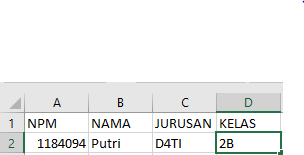
\includegraphics{gambar/csv1.jpg}
\item Save file dengan format CSV kemudian file terbuat.\\
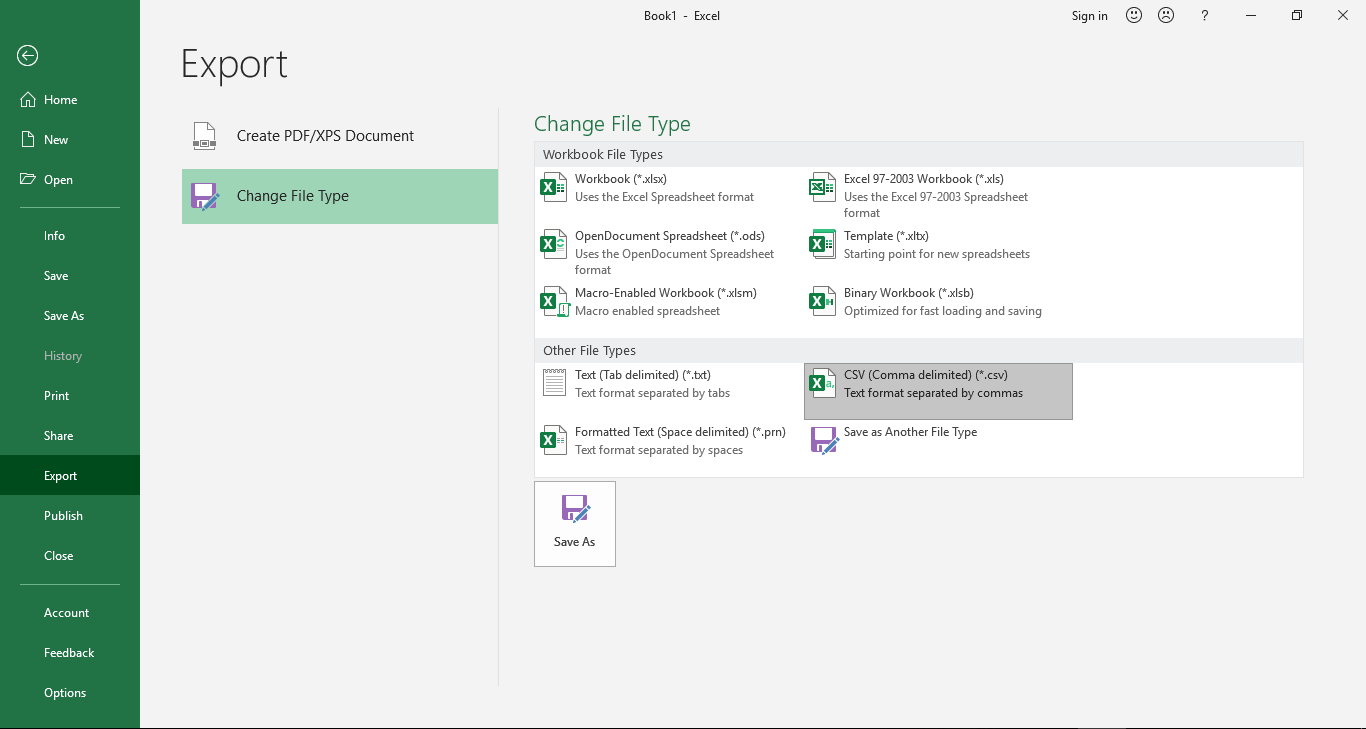
\includegraphics[scale = 0.3]{gambar/csv2.jpg}
\end{enumerate}


\item Sejarah Library CSV\\
Format CSV(Comma Separated Value) merupakan format ekspor impor yang paling sering digunakan untuk Database dan spreadsheet. CSV menggunakan format standar pada RCF 4180. Pada CSV sering terjadi perbedaan format dalam data yang dibuat dan digunakan menggunakan aplikasi yang berbeda yang disebabkan karena kurangnya standarisasi yang didefinisikan dengan baik. Hal ini paling sering membuat proggramer mengatakan "Buat data ini seperti pada Excel".

\item Sejarah Library Pandas\\
Pandas adalah alat sebagai analisis data dan struktur bahasa pemrograman python. Pandas Dapat digunakan untuk mengolah data dengan mudah. salah satu fitur pada pandas adalah Dataframe. Fitur ini membuat kita dapat membaca sebuah file dan membuatnya menjadi table. Banyak file yang dapat dibaca dengan menggunakan Pandas, seperti file .txt, .csv, .tsv, dan masih banyak lagi.

\item Fungsi Fungsi pada Library CSV\\
\begin{enumerate}
\item Fungsi Reader: untuk membaca isi file CSV dari list.\\
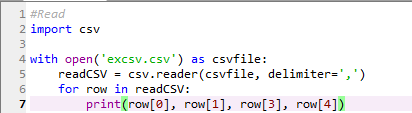
\includegraphics[scale = 0.7]{gambar/csv3.jpg}

\item DictReader: untuk membaca isi file  CSV dari Dictionary.\\
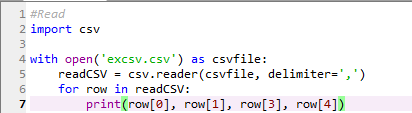
\includegraphics[scale = 0.7]{gambar/csv3.jpg}

\item write: untuk menulis file  CSV dari list.\\
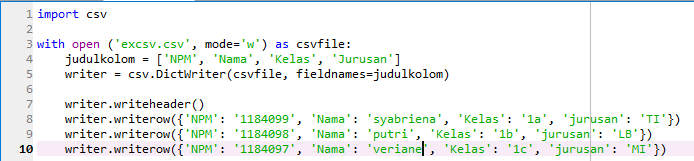
\includegraphics[scale = 0.5]{gambar/csv4.jpg}

\item DictWrite: untuk menulis file CSV dari Dictionary.\\
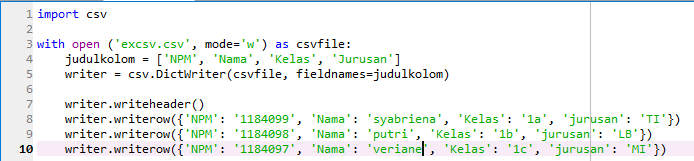
\includegraphics[scale = 0.5]{gambar/csv4.jpg}
\end{enumerate}

\item Fungsi Fungsi pada Library Pandas\\
\begin{enumerate}

\item read CSV: Untuk membaca file CSV\\
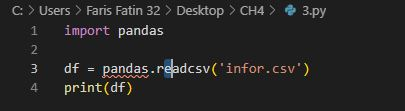
\includegraphics{gambar/csv5.jpg}

\item to CSV: Untuk menulis file CSV\\
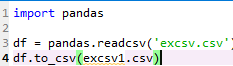
\includegraphics{gambar/csv6.jpg}
\end{enumerate}

\end{enumerate}

\section{Keterampilan Pemrograman}
\begin{enumerate}

\item Buatlah fungsi untuk membuka file csv dengan lib csv mode list.\\ %1
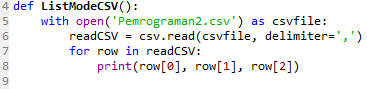
\includegraphics{gambar/csv7.jpg}

\item Buatlah fungsi untuk membuka file csv dengan lib csv mode dictionary.\\ %2
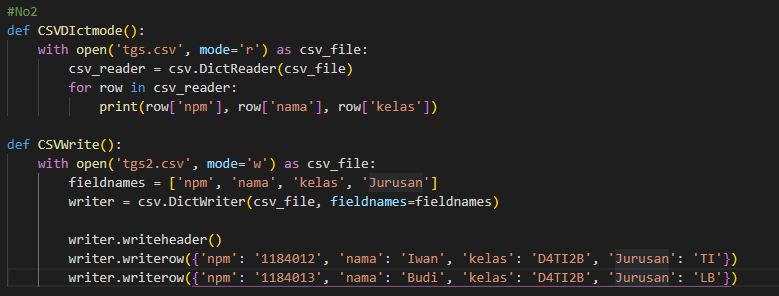
\includegraphics[scale = 0.7]{gambar/csv8.jpg}

\item Buatlah fungsi untuk membuka file csv dengan lib pandas mode list.\\ %3
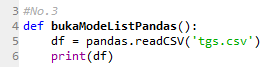
\includegraphics{gambar/csv9.jpg}

\item Buatlah fungsi untuk membuka file csv dengan lib pandas mode Dictionary.\\ %4
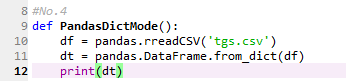
\includegraphics{gambar/csv10.jpg}

\item Buatlah fungsi baru di NPM pandas.py untuk mengubah format tanggal menjadi standar dataframe.\\ %5
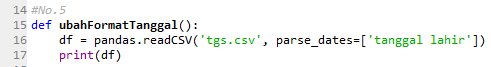
\includegraphics{gambar/csv11.jpg}

\item Buatlah fungsi baru di NPM pandas.py untuk mengubah index kolom.\\ %6
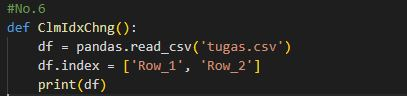
\includegraphics{gambar/csv12.jpg}

\item Buatlah fungsi baru di NPM pandas.py untuk mengubah atribut atau nama kolom.\\ %7
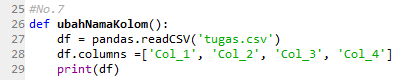
\includegraphics{gambar/csv13.jpg}

\item Buat program  main.py yang menggunakan library NPM csv.py yang membuat dan membaca file csv.\\ %8
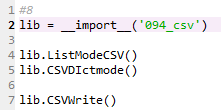
\includegraphics{gambar/csv14.jpg}

\item Buatlah program  main2.py yang menggunakan library NPM pandas.py yang membuat dan membaca file csv.\\ %9
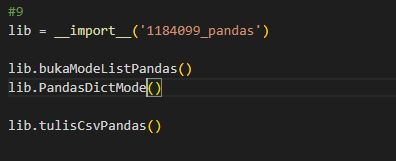
\includegraphics{gambar/csv15.jpg}

\end{enumerate}
%\begin{enumerate}
%\end{enumerate}

\section{Keterampilan Penanganan Error}
TypeError: NPM2() takes 0 positional arguments but 1 was given \\
solusi: Menambahkan argument pada NPM2().\\


Try Except:
\lstinputlisting[language=Python]{src/tryexcept.py}





